\documentclass{beamer}

%\usepackage{graphicx}
\usepackage{caption}
\captionsetup[figure]{labelformat=empty}% redefines the caption setup of the figures environment in the beamer class
%\captionsetup[figure]{labelformat=empty,labelsep=none}

\usetheme[everytitleformat=regular]{m}

%\usepackage{booktabs}
%\usepackage[scale=2]{ccicons}

\title{Deep Learning for Image Anomaly Detection}
%\subtitle{A modern beamer theme}
\date{August 10, 2015}

\author{Jesse Berwald \and Janet Keel \\ 
        Ross Churchley \and Omeiza Olumoye \and Pawan Patel \\ 
        Jonathan Smith \and Parker Williams \and Ruiyu Yang \\\\}

%\institute[shortinst]{\inst{1} Affil1 \and \inst{2} Affil2 \and \inst{3} Affil3}

%\institute{Institute or miscellaneous information}

% \titlegraphic{\hfill
\includegraphics[height=1.5cm]{logo/logo}}
\graphicspath{{Pics_for_Presentation/}}

\begin{document}

\maketitle

\begin{frame}
  \frametitle{Table of Contents}
  \setbeamertemplate{section in toc}[sections numbered]
  \tableofcontents[hideallsubsections]
\end{frame}

\section{Introduction}

\begin{frame}

    \frametitle{Goal of This Project}

	One of the issues facing industries that deal with large numbers of digital photographs, such as magazines and retailers, is photo accuracy. Most of these photos undergo some form of editing(``Photoshopping"). Detecting anomalies automatically in such cases would enable retailers such as Target to filter out mistakes before they enter production. By training a modern deep convolution neural network [1,5] on a collection of correct images within a narrow category, we would like to construct a network which will learn to recognize well-edited images. \\


\end{frame}


\begin{frame}[fragile]

  \frametitle{Some Anomaly Figures}
  \begin{columns}[onlytextwidth]
  \begin{column}{.45\textwidth}
  \begin{figure}
  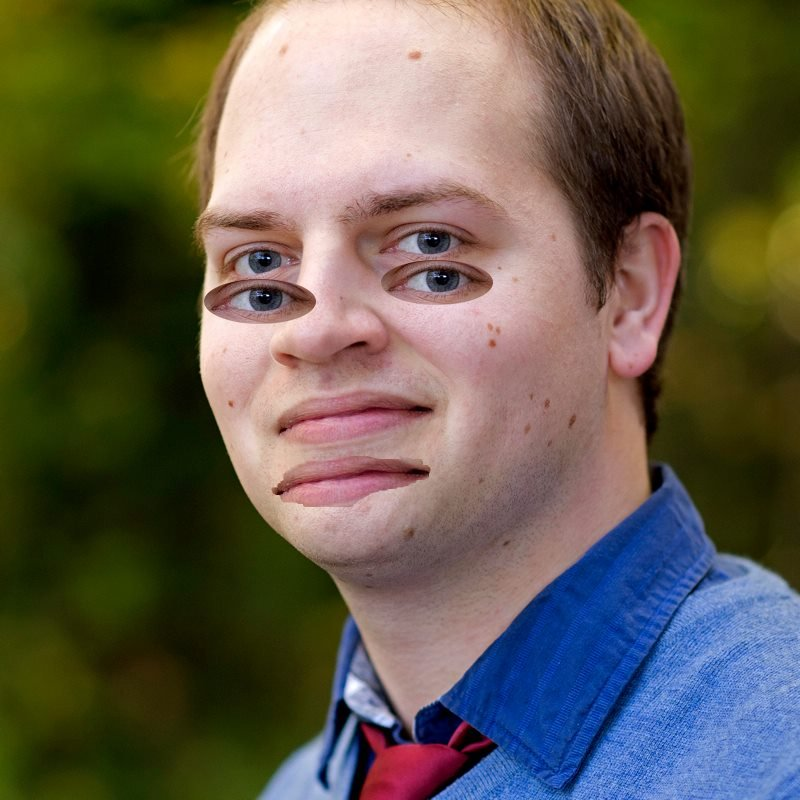
\includegraphics[width=\textwidth,height=0.5\textheight]{1475772_10202006969609191_901353218_n}
  \end{figure}
  \end{column}
  \hfill
  \begin{column}{.45\textwidth}
  \begin{figure}
  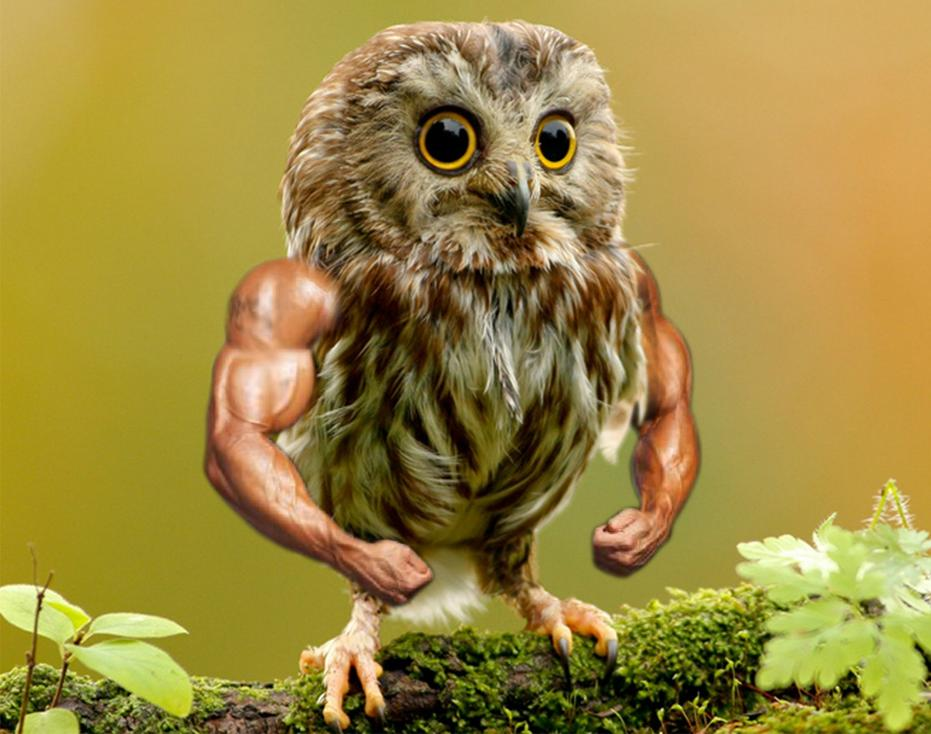
\includegraphics[width=\textwidth,height=0.5\textheight]{OwlWithArms}
  \end{figure}
  \end{column}
\end{columns}

\end{frame}


\section{Image Collection Process}

\begin{frame}
  \frametitle{Image Collection}
    \alert{Process}
    \begin{itemize}
    \item In order to train the neural network, we need \emph{lots} of images
    \item On the order of tens of thousands, probably even more!
    \item We collect our images from Flickr, using the Flickr API, and crop/resize them to a common size (256x256)
    \end{itemize}
    \alert{Teaching a Machine} \\
    The general idea is as follows: We feed the machine N ``good" images and N ``bad" images, and we tell it which are which. It will eventually learn how to identify these images and be able to independently identify the good from the bad.

\end{frame}

\begin{frame}[fragile]
  \frametitle{Image Processing}

	\begin{columns}
	\begin{column}{.32\textwidth}
	\begin{figure}
	  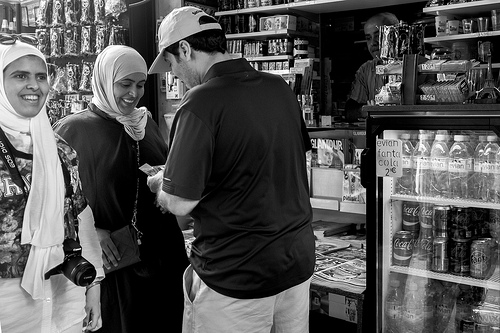
\includegraphics[width=\textwidth,height=0.45\textheight]{20441017631[1]}
	\end{figure}
	\end{column}
	\begin{column}{.32\textwidth}
	\begin{figure}
	  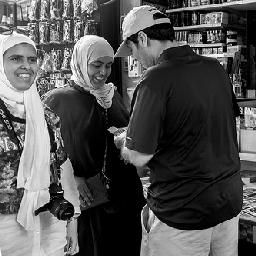
\includegraphics[width=\textwidth,height=0.45\textheight]{20441017631[2]}
	\end{figure}
	\end{column}
	%\hfill
	\begin{column}{.32\textwidth}
	\begin{figure}
	  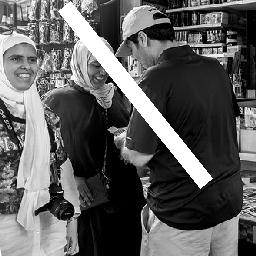
\includegraphics[width=\textwidth,height=0.45\textheight]{20441017631}
	\end{figure}
	\end{column}
	\end{columns}

\end{frame}


\section{Learning Process}
\begin{frame}

    \frametitle{Network Structure}
    \begin{center}
    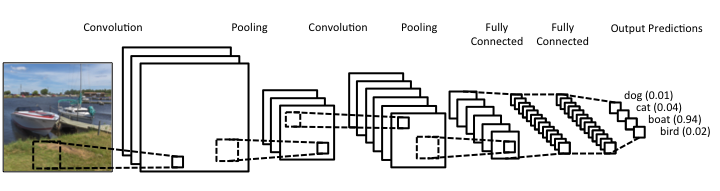
\includegraphics[width=0.75\textwidth]{ConvolutionalNeuralNetwork.png} \\
    \begin{tiny}
    Structure of a Convolutional Neural Network
    \end{tiny}
    \end{center}
    \begin{itemize}
    \item Begin with original image
    \item Apply convolution filter + maximum pooling filter
    \item Repeat
    \item Apply two fully connected layers
    \item End with only a small number of values
    \end{itemize}

\end{frame}


\begin{frame}

    \frametitle{Convolution Filter}
    \begin{center}
    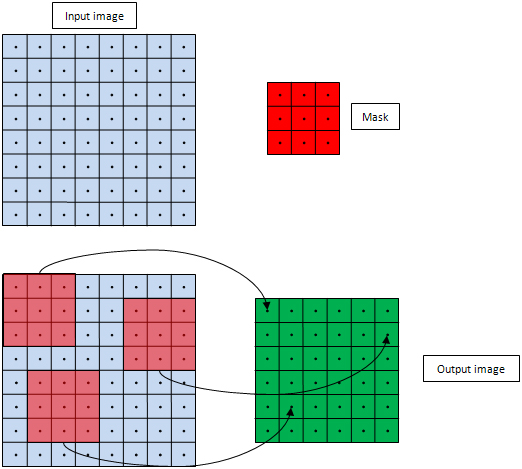
\includegraphics[width=0.40\textwidth]{ConvolutionFilter.jpeg} \\
    \begin{tiny}
    Basic Structure of Convolution Filter
    \end{tiny}
    \end{center}
    \begin{itemize}
    \item Used for feature extraction
    \item Weights for mask/filter are initialized randomly and gradually learned
    \end{itemize}
    
\end{frame}


\begin{frame}

	\frametitle{Max Pooling Filter}
    \begin{center}
	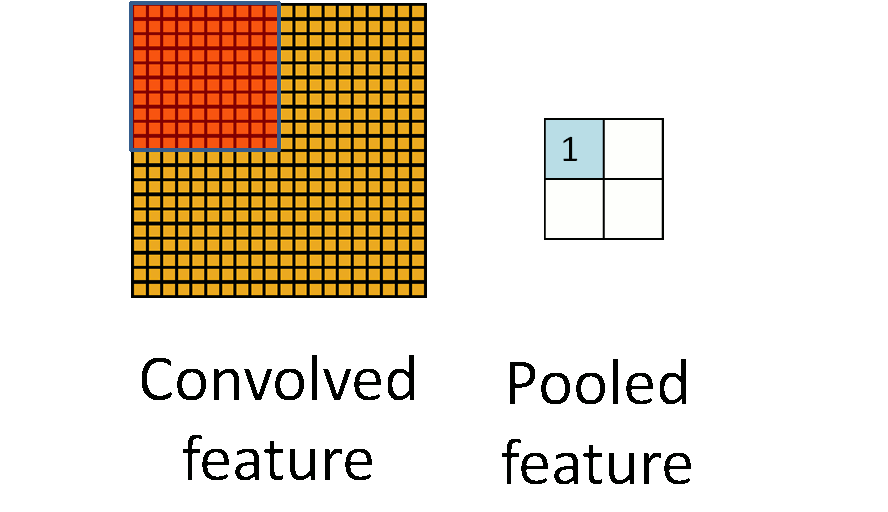
\includegraphics[width=0.40\textwidth]{Pooling_schematic-0.png}
	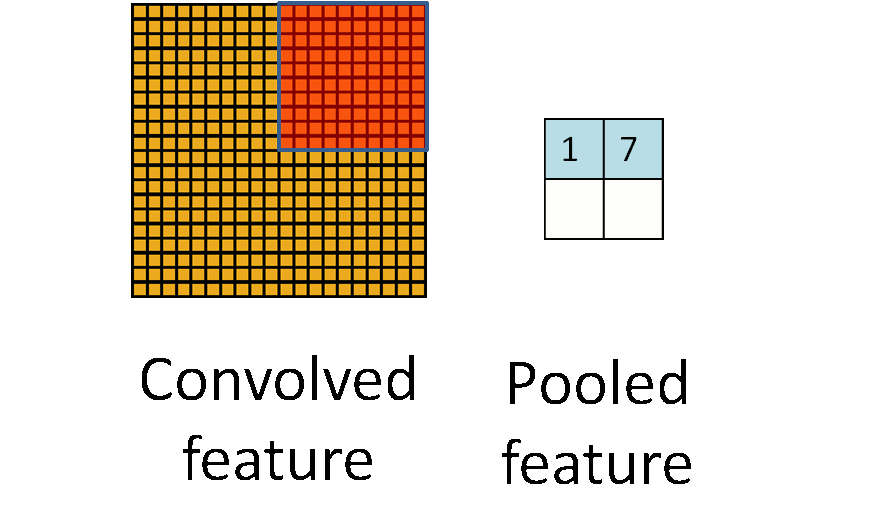
\includegraphics[width=0.40\textwidth]{Pooling_schematic-1.png} \\
	\begin{tiny}
	Basic Structure of Pooling Filter
	\end{tiny}
	\end{center}
	\begin{itemize}
	\item Used for summarizing data
	\item Takes the maximum value in each sub-block of the convoluted image
	\item Used in tandem with the convolution filter, extracts the most prominent feature in a sub-block
	\end{itemize}
    
\end{frame}

\begin{frame}

    \frametitle{Error Reduction}
    How do we go about reducing error?
    \begin{itemize}
    \item Think of error as a function of all initially randomized parameters
    \item $error = E_{input}(weights)$
    \item Calculate error for a given batch of input images
    \item Adjust the parameters along $\nabla E$
    \item In other words, for a learning rate $\alpha$, we update a set of parameters $W$ as follows:
    \end{itemize}
    \begin{equation*}
    W_{i+1} = W_i - \alpha \nabla E(W_i)
    \end{equation*}
    
\end{frame}



\begin{frame}

    \frametitle{Current Status and Future Work}
     \begin{itemize}
    \item The current network is in the development stage
    \item We are running it on a set of $\sim$4000 images, with plans to test on much larger data sets
    \item These images are ``anomalized" by drawing a white line of random length to imitate an overzealous eraser
    \item The same framework may be used to detect more complicated or specific anomalies once we get the initial run working
    \end{itemize}
    
\end{frame}


%\section{Contents}

% \begin{frame}[fragile]
%   \frametitle{More Figures}

% \begin{columns}[onlytextwidth]
% \begin{column}{.45\textwidth}
% \begin{figure}
%   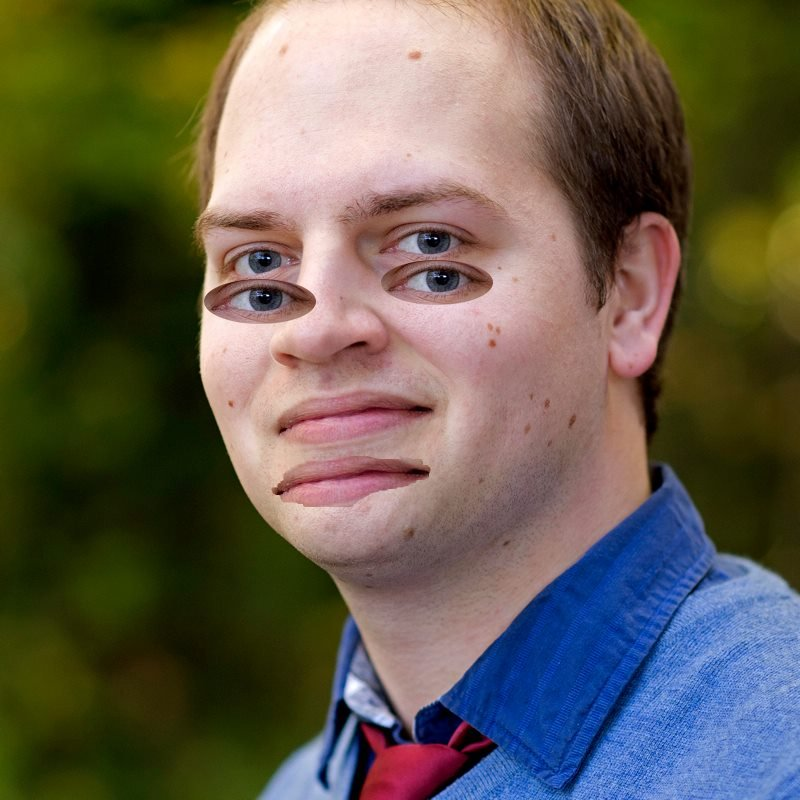
\includegraphics[width=\textwidth,height=0.5\textheight]{1475772_10202006969609191_901353218_n}
%   \caption{First image}
% \end{figure}
% \end{column}
% \hfill
% \begin{column}{.45\textwidth}
% \begin{figure}
%   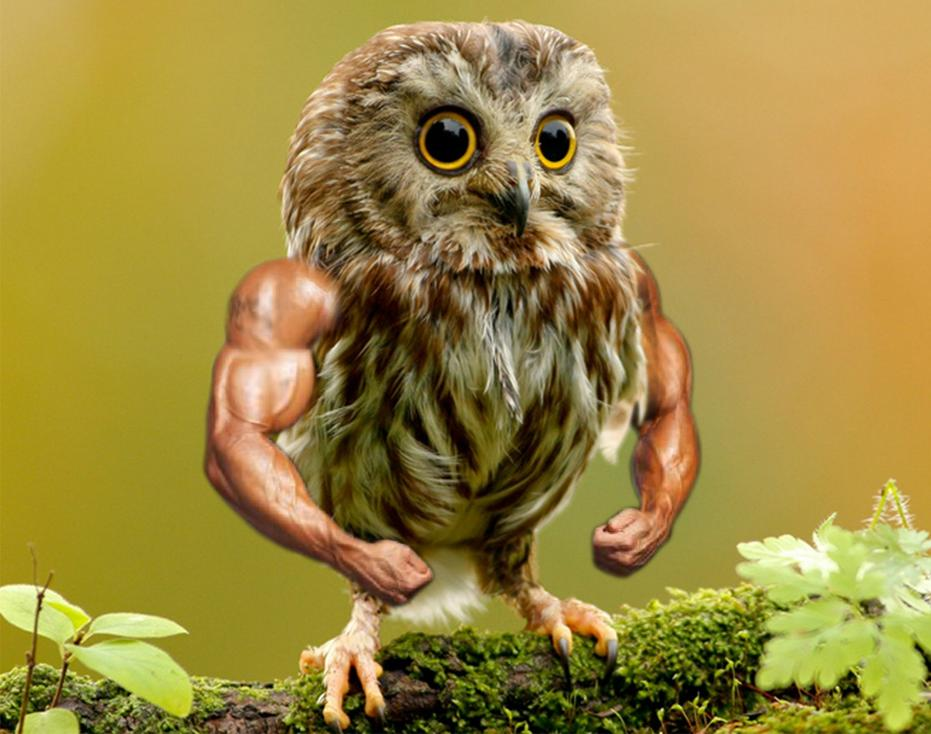
\includegraphics[width=\textwidth,height=0.5\textheight]{OwlWithArms}
%   \caption{Second image}
% \end{figure}
% \end{column}
% \end{columns}

% \end{frame}

%\section{Conclusion}

\begin{frame}[fragile]
  \frametitle{References}
  
  \begin{center}
  \begin{tabular}{lp{9.0cm}} 
    \text{[1]} & Going Deeper with Convolutions, http://arxiv.org/abs/1409.4842  \\
    \text{[2]} & Spatial Pyramid Pooling in Deep Convolutional Networks for Visual Recognition, http://arxiv.org/pdf/1406.4729v1.pdf \\
    \text{[3]} & http://googleresearch.blogspot.com/2014/09/building-deeper-understandingof-images.html \\
    \text{[4]} & Google: “famous photoshop fails”  \\
    \text{[5]} & Delving Deep into Rectifiers: Surpassing Human-Level Performance on Image Net Classification, http://arxiv.org/pdf/1502.01852v1.pdf \\
  \end{tabular}
  \end{center}
   %   Additional references
   % [*] http://www.pyimagesearch.com/2014/10/13/deep-learning-amazon-ec2-gpu-python-nolearn/
   % [*] http://www.wired.com/2013/05/neuro-artificial-intelligence/
   % [*] http://www.slideshare.net/0xdata/h2o-distributed-deep-learning-by-arno-candel–071614

\end{frame}



% \begin{frame}{Summary}

%   Get the source of this theme and the demo presentation from

%   \begin{center}\url{github.com/matze/mtheme}\end{center}

%   The theme \emph{itself} is licensed under a
%   \href{http://creativecommons.org/licenses/by-sa/4.0/}{Creative Commons
%   Attribution-ShareAlike 4.0 International License}.

%   \begin{center}\ccbysa\end{center}

% \end{frame}

% \plain{Questions?}

% \begin{frame}[allowframebreaks]

%   \frametitle{References}

%   \bibliography{demo}
%   \bibliographystyle{abbrv}

% \end{frame}


\end{document}
